%-------------------------------------------------------------------------
% Design Project Input/Output Module Description
%-------------------------------------------------------------------------

\clearpage
\section{Servo Output Module}
\label{sec-output-servo}

This output module enables your IoT device to control a high-torque
standard servo. Servos are useful for interfacing directly with the
environment; for example, servos can tilt, rotate, push other objects,
or flip switches. Servos can be large or small, but the servo you will
use is a standard servo that is useful in IoT environments. The position
of the servo motor is set by the length of a pulse, and the servo
expects to receive a pulse roughly every \wu{20}{ms}. If the Arduino
sends a pulse that is high for \wu{1}{ms}, then the servo angle will be
zero; if it is \wu{1.5}{ms}, then it will be at its center position, and
if it is \wu{2}{ms} it will be at 180 degrees. The motor can rotate 180
degrees at max speed in about half a second, but slower and more
fine-tuned turning is possible as well.

A sample circuit and Arduino code is shown below to get you started.
Note that the servo's ribbon wire has red, brown, and yellow wires. Red
is power, while brown is ground, and yellow is used to control the servo
from the Arduino. The \wu{470}{uF} capacitor ensures a steady power
supply to the Arduino. Make sure the longer lead of the capacitor is
connected to power while the shorter lead is connected to ground.  The
example code will sweep the servo position between 0 and 180 degrees
back and forth. After setting up the circuit and programming the
Arduino, check that the servo is sweeping back and forth steadily
between 0 and 180 degrees. You can then attach arms or horns to the
servo to control other objects and place the servo itself in more
strategic locations. Also try experimenting with smaller delays by
replacing \TT{delay(15)} with a smaller number like 5. What happens when
you try this and could it be useful?

\vspace{0.1in}
\begin{minipage}[t]{0.49\tw}
  \vspace{0.0in}
  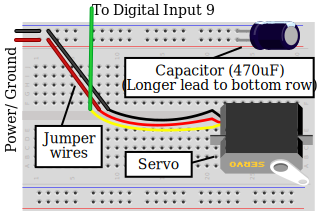
\includegraphics[width=\tw]{output-servo-annotated.svg.pdf}
\end{minipage}
\hspace{0.1in}
\begin{minipage}[t]{0.49\tw}
  \vspace{0.1in}
  \begin{Verbatim}[gobble=3,fontsize=\small]
    #include <Servo.h>

    int pin_servo = 6;

    Servo servo;
    int servo_angle = 0; // Servo position in degrees

    void setup() {
      servo.attach(pin_servo);
    }

    void loop() {
      // Scan from 0 to 180 degrees

      for( servo_angle = 0; servo_angle < 180; servo_angle++ ) {
        servo.write( servo_angle );
        delay(15);
      }

      // Scan back from 180 to 0 degrees

      for( servo_angle = 180; servo_angle > 0; servo_angle-- ) {
        servo.write( servo_angle );
        delay(15);
      }
    }
  \end{Verbatim}
\end{minipage}
\vspace{0.1in}

%Questions:
